\documentclass[a4paper, 12pt]{article}

\usepackage[utf8]{inputenc}
\usepackage{amsmath}
\usepackage{indentfirst}
\usepackage{graphicx}
\usepackage{multicol,lipsum}
\usepackage{hyperref}
\usepackage{minted}
\usepackage{cancel}

\begin{document}
%\maketitle

\begin{titlepage}
	\begin{center}
	
	%\begin{figure}[!ht]
	%\centering
	%\includegraphics[width=2cm]{c:/ufba.jpg}
	%\end{figure}

		\Huge{Instituto de Ciências Matemáticas e de Computação}\\
		\large{Departamento de Ciências de Computação}\\ 
		\large{SCC0503 - Algoritmos e Estruturas de Dados II}\\ 
		\vspace{15pt}
        \vspace{95pt}
        \textbf{\LARGE{Relatório Exercício 07}}\\
		%\title{{\large{Título}}}
		\vspace{3,5cm}
	\end{center}
	
	\begin{flushleft}
		\begin{tabbing}
			Alunos: Ryan Souza Sá Teles, Silmar Pereira da Silva Junior \\
            NUSP's: 12822062, 12623950.
			Professor: Leonardo Tórtoro Pereira\\
			%Professor co-orientador: \\
	\end{tabbing}
 \end{flushleft}
	\vspace{1cm}
	
	\begin{center}
		\vspace{\fill}
			 Julho\\
		 2022
			\end{center}
\end{titlepage}
%%%%%%%%%%%%%%%%%%%%%%%%%%%%%%%%%%%%%%%%%%%%%%%%%%%%%%%%%%%

\newpage
% % % % % % % % % % % % % % % % % % % % % % % % % %
\newpage
\tableofcontents
\thispagestyle{empty}

\newpage
\pagenumbering{arabic}
% % % % % % % % % % % % % % % % % % % % % % % % % % %
\section{Introdução}
Com o sucesso na aplicação de vaga da empresa BugSoft, o desenvolvimento do novo jogo: Credo dos Frita Sinos pode ser complementada, deste modo, com os algoritmos de Triangulação de Delaunay e de pathfinding o jogo ficará completo.

\newpage
\section{Desenvolvimento}

O desenvolvimento do projeto fez uso das abstrações já adotadas em sala de aula e o modelo de dígrafo selecionado para trabalhar na construção das dungeons foi o de "matriz de adjâcencias".\\

Tal decisão foi tomada pela comparação entre a complexidade das operações em comparação com a alternativa (lista de adjacências) e a frequência com que essas operações são feitas.\\
A principail operação realizada durante o algoritimo é a adição de vertices e arestas, em que a lista é O(1) em ambos, já a matriz é $O(|V|^2)$ e O(1) respectivamente. Com relação as demais ambas as abordagens tem complexidades semelhantes.\\
Outro fator que corroborou para a escolha foi a complexidade de espaço entre as opções, com a lista sendo $O(|V|+|E|)$ enquanto a matrix de adjacências sendo $O(|V|^2)$.\\

O algoritmo de Prim já implementado em sala de aula foi utilizado para "limpar" as arestas das dungeons recem criadas, de modo a garantir somente uma aresta entre uma sala e outra.

Para limpar as arestas, foi necessário utilizar o array de Predecessores gerado pelo algortimo de prim, com ele, foi implementado um metódo dentro de uma nova classe, GraphConverter, nela, foi gerado uma nova dungeon e alem disso, calculada a distancia entre cada sala por meio da distância euclidiana entre os pontos (vertíces).\\

O método para calculo de distância foi implementado na classe abstrata Abstract Graph, essa decisão foi feita devido a complexidade e quantidade de conflitos gerados ao abstrair uma classe chamada Dungeon, onde deveria conter tal método, em diversos pontos do código é chamado DigraphMatrix e GraphMatrix, gerando erros.\\


Com o objetivo de aplicar as boas práticas de código na atividade, uma nova package chamada dungeons foi criada para abrigar as classes referentes a criação de dungeon, deste modo, a organização do código se mantém.\\

Para a impressão da distância entre cada sala, foi utilizado os algoritmos Breadth First Search, Depth First Search e A*, quais somente o último não foi implementado em sala de aula.

Abaixo, as implementações:\\

Implementação da classe GraphConverter (Classe qual possui o método que converte a lista de predecessores do algoritmo de prim para um grafo):


\begin{minted}[mathescape, linenos]{java}
public class GraphConverter {
    private GraphConverter() {}
    public static AbstractGraph predecessorListToGraph(AbstractGraph dungeon, int[] predecessor){
        AbstractGraph newDungeon = new DigraphMatrix();

        Room newRoom;
        for (int i = 0; i < dungeon.getNumberOfVertices(); i++) {
            newRoom = (Room)dungeon.getVertices().get(i);
            newDungeon.addVertex(newRoom);
        }

        float distance;
        Room source;
        Room destination;
        for (int i = 1; i < predecessor.length; i++) {
            source = (Room)dungeon.getVertices().get(predecessor[i]);
            destination = (Room)dungeon.getVertices().get(i);
            distance = dungeon.calcEuclidianDistance(source, destination);
            newDungeon.addEdge(source, destination, distance);
            newDungeon.addEdge(destination, source, distance);
        }
        return newDungeon;
    }
}
\end{minted}


\begin{minted}[mathescape, linenos]{java}
  
\end{minted}

Implementação do método calcEuclidianDistance:

\begin{minted}[mathescape, linenos]{java}
public float calcEuclidianDistance(Room source, Room destination) {
    int x1 = (int) source.getRoom().getX();
    int y1 = (int) source.getRoom().getY();
    int x2 = (int) destination.getRoom().getX();
    int y2 = (int) destination.getRoom().getY();
    return (float) Math.sqrt(Math.pow(x1 - x2, 2) + Math.pow(y1 - y2, 2));
}
\end{minted}

Implementação do Algoritmo A*

\begin{minted}[mathescape, linenos]{java}
public final class AStarTraversal extends TraversalStrategy {
    private final List<Vertex> verticesToVisit;
    private final float[] vertexHeuristic;

    public AStarTraversal(AbstractGraph graph) {
        super(graph);
        verticesToVisit = new LinkedList<>();
        vertexHeuristic = new float[getGraph().getNumberOfVertices()];
        Arrays.fill(vertexHeuristic, Float.POSITIVE_INFINITY);
    }

    public void traverseGraph(Vertex source) {
        throw new UnsupportedOperationException("Not implemented yet");
    }

    public void traverseGraph(Vertex source, Vertex destination) {
        var sourceIndex = getGraph().getVertices().indexOf(source);
        vertexHeuristic[sourceIndex] = getHeuristicDistance((Room) source, (Room) destination);
        setDistanceToVertex(sourceIndex, 0);
        var visitedVertex = new LinkedList<>();
        verticesToVisit.add(source);

        var currentVisitedVertex = source;
        var currentVisitedVertexIndex = getGraph().getVertices().indexOf(currentVisitedVertex);
        while (currentVisitedVertex != destination && !verticesToVisit.isEmpty()) {
            if (currentVisitedVertex != null) {
                var adjacentVertex = getGraph().getFirstConnectedVertex(currentVisitedVertex);
                while (adjacentVertex != null) {
                    var adjacentVertexIndex = getGraph().getVertices().indexOf(adjacentVertex);
                    var currentDistance = getDistanceToVertex(currentVisitedVertexIndex) + getTrueDistance((Room) currentVisitedVertex, (Room) adjacentVertex);
                    setDistanceToVertex(adjacentVertexIndex, currentDistance);
                    if (!visitedVertex.contains(adjacentVertex)) {
                        vertexHeuristic[adjacentVertexIndex] = currentDistance + getHeuristicDistance((Room) adjacentVertex, (Room) destination);
                        verticesToVisit.add(adjacentVertex);
                    }
                    adjacentVertex = getGraph().getNextConnectedVertex(currentVisitedVertex, adjacentVertex);
                }
            }
            currentVisitedVertex = getVertexWithBestHeuristic();
            if (currentVisitedVertex == null)
                break;
            currentVisitedVertexIndex = getGraph().getVertices().indexOf(currentVisitedVertex);
            visitedVertex.add(currentVisitedVertex);
            verticesToVisit.remove(currentVisitedVertex);

        }
        printDistances();
    }

    private Vertex getVertexWithBestHeuristic() {
        return verticesToVisit.stream().min((vertexOne, vertexTwo) -> {
            var vertexOneIndex = getGraph().getVertices().indexOf(vertexOne);
            var vertexTwoIndex = getGraph().getVertices().indexOf(vertexTwo);
            var distance1 = vertexHeuristic[vertexOneIndex];
            var distance2 = vertexHeuristic[vertexTwoIndex];
            return Float.compare(distance1, distance2);
        }).orElse(null);
    }

    private float getHeuristicDistance(Room source, Room destination) {
        //euclidean Distance
        var x1 = source.getPoint().getX();
        var y1 = source.getPoint().getY();
        var x2 = destination.getPoint().getX();
        var y2 = destination.getPoint().getY();
        return (float) Math.sqrt(Math.pow(x1 - x2, 2) + Math.pow(y1 - y2, 2));
    }

    private float getTrueDistance(Room source, Room destination) {
        //manhattan Distance
        var x1 = source.getPoint().getX();
        var y1 = source.getPoint().getY();
        var x2 = destination.getPoint().getX();
        var y2 = destination.getPoint().getY();
        return (float) Math.abs(x1 - x2) + (float) Math.abs(y1 - y2);
    }
}
\end{minted}

Implementação da Main (lógica do programa)

\begin{minted}[mathescape, linenos]{java}
private static final int NUMBER_OF_LOCKS = 2;

public static void main(String[] args) {
    Scanner scanner = new Scanner(System.in);
    int randomSeed = scanner.nextInt();
    scanner.nextLine();
    int numberRooms = scanner.nextInt();

    AbstractGraph dungeon = generateDungeonLevel(randomSeed, numberRooms);
    setSpecialRooms(dungeon);
    setKeylocksRooms(dungeon);

    printDungeonWithDFS(dungeon);
    printDungeonWithBFS(dungeon);
    printDungeonWithAStar(dungeon);
    SwingUtilities.invokeLater(() -> new DungeonGraphic(dungeon).setVisible(true));
}
\end{minted}

Implementação dos submétodos da Main:

\begin{minted}[mathescape, linenos]{java}
private static void setKeylocksRooms(AbstractGraph dungeon) {
        var keylockTraverse = new KeyLockGenerator(dungeon,NUMBER_OF_LOCKS);
        keylockTraverse.traverseGraph(dungeon.getEntrance());
    }

    private static void setSpecialRooms(AbstractGraph dungeon) {
        FloydWarshallTraversal floydWarshallTraversal = new FloydWarshallTraversal(dungeon);
        floydWarshallTraversal.traverseGraph(null);
        Room centralRoom= (Room) floydWarshallTraversal.getCentralVertex();
        centralRoom.setCheckPoint(true);
        Room startRoom= (Room) floydWarshallTraversal.getPeripheralVertex();
        startRoom.setEntrance(true);
        dungeon.setEntrance(startRoom);
        Room exitRoom = (Room) floydWarshallTraversal.getFarthestVertexFrom(startRoom);
        exitRoom.setExit(true);
        dungeon.setExit(exitRoom);
    }

    private static void printDungeonWithAStar(AbstractGraph dungeon) {
        var aStar = new AStarTraversal(dungeon);
        aStar.traverseGraph(dungeon.getEntrance(),dungeon.getExit());
    }

    private static void printDungeonWithDFS(AbstractGraph dungeon) {
        var depthFirstTraversal = new DepthFirstTraversal(dungeon);
        depthFirstTraversal.traverseGraph(dungeon.getEntrance());
    }

    private static void printDungeonWithBFS(AbstractGraph dungeon) {
        var breadthFirstTraversal = new BreadthFirstTraversal(dungeon);
        breadthFirstTraversal.traverseGraph(dungeon.getEntrance());
    }

    private static AbstractGraph generateDungeonLevel(int randomSeed, int numberRooms) {
        RandomSingleton.getInstance(randomSeed); //Inicializar gerador de números aleatórios
        var randomDungeonGenerator = new RandomDungeonGenerator(numberRooms); //Gerar 20 salas
        var dungeon = randomDungeonGenerator.getDungeon(); //Pegar o grafo com salas
        DelaunayTriangulation.triangulateGraphVertices(dungeon); //Criar arestas

        int[] predecessorIndexList = cleanEdgesAndGetPredecessorList(dungeon);

        return GraphConverter.predecessorListToGraph(dungeon, predecessorIndexList);
    }

    private static int[] cleanEdgesAndGetPredecessorList(AbstractGraph dungeon) {
        var primTraversal = new PrimMSTTraversal(dungeon);
        primTraversal.traverseGraph(dungeon.getVertices().get(0));
        return primTraversal.getPredecessorArray();
    }
\end{minted}

\newpage
\section{Resultados}
\graphicspath{ {./Results/} }
Como resultados obtemos:\\

Semente: 5

Numero de Salas: 25

temos:\\
\\
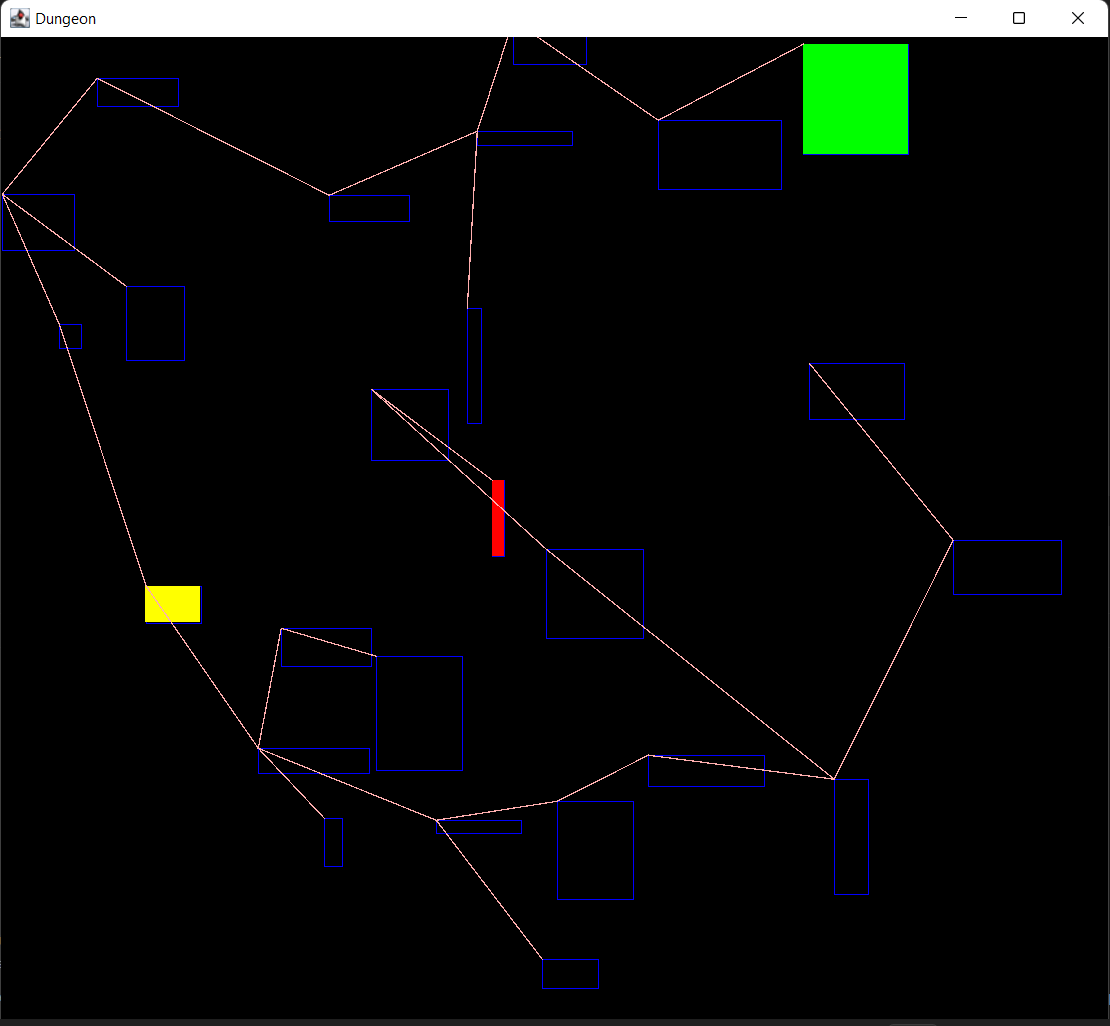
\includegraphics[width=\textwidth]{Grafo1.png}\\

Semente: 3

Numero de Salas: 12

temos:\\
\\
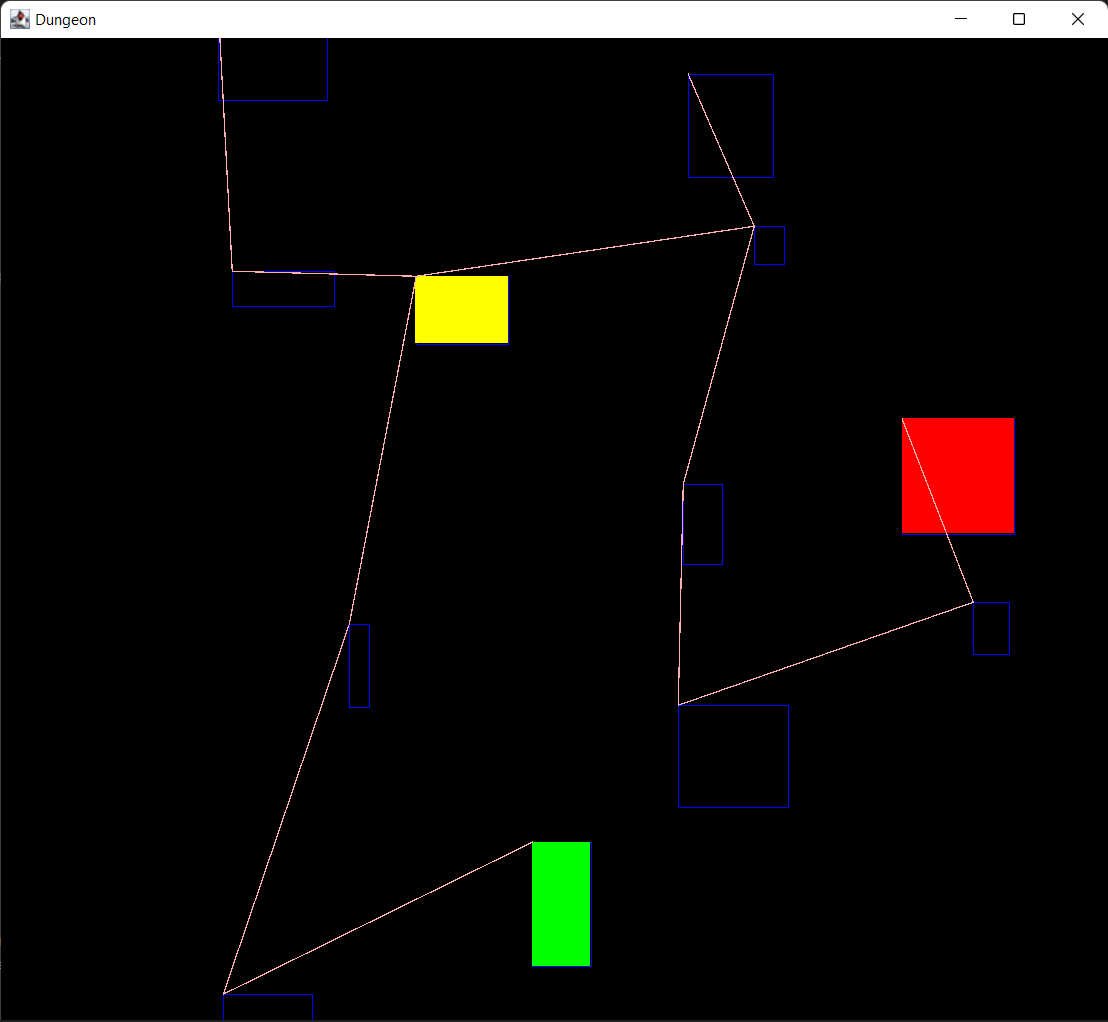
\includegraphics[width=\textwidth]{Grafo2.png}\\

Semente: 9

Numero de Salas: 49

temos:\\
\\
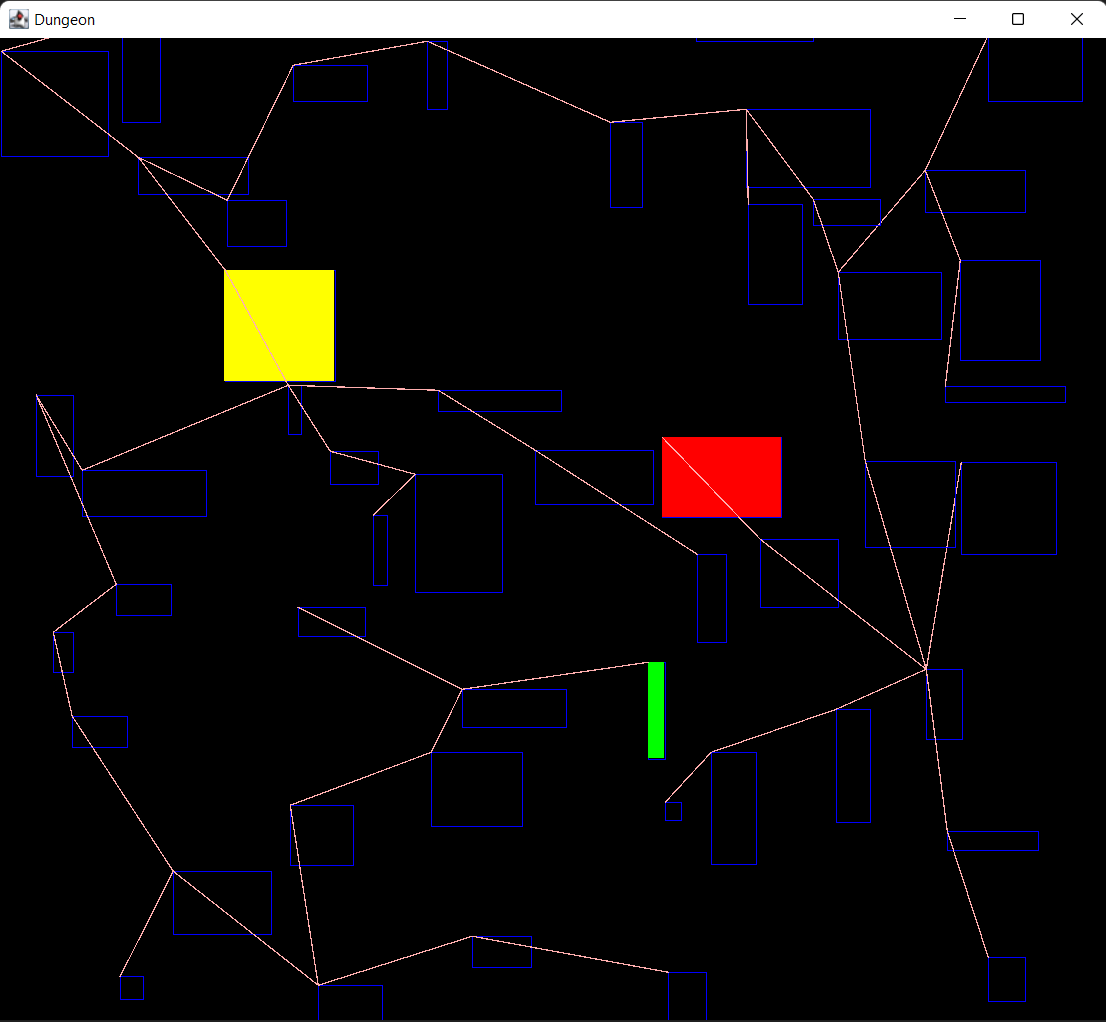
\includegraphics[width=\textwidth]{Grafo3.png}\\

\end{document}



